\documentclass{article}
\usepackage{graphicx} % Required for inserting images

\title{My wonderful HRI task \\
Elective in AI / HRI Report}
\author{Name and matricola of all authors}
\date{}


\begin{document}

\maketitle

All students have equally contributed to the project (or a different statement highlighting specific contributions)

\section{Introduction}

\subsection{Context and motivation}

What is the context of the project (e.g., robot in a restaurant, at school, etc.)

Why should we produce such technology (benefits for the society, economy, ...)?


\subsection{Objectives}
\label{sec:obj}

Specific objective of the project:
example, demonstrating this social ability of the robot when dealing with this HRI task

\subsection{Summary of the results}

In the project, we have demonstrated/shown that  ....



\section{Related work}

Which papers \cite{HRIpaper}, seminars \cite{HRIseminar}, lecture slides \cite{HRIslides}  inspired this project?

What do you want to show/test with respect to what you have learned reading papers/listening to lectures and seminars?

Is your work original with respect to the state of the art, or do you want to confirm some existing result in a different case?


\section{Solution}

\begin{figure}
    \centering
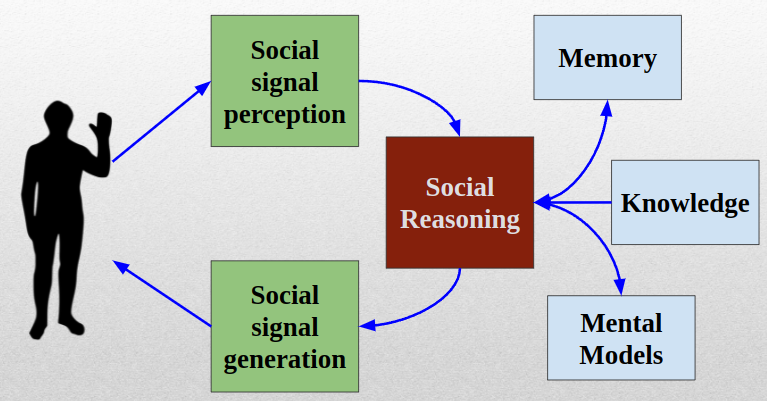
\includegraphics[width=0.9\textwidth]{HRI_arch.png}
    \caption{Architecture (TO BE MODIFIED!!!)}
    \label{fig:arch}
\end{figure}

Functional architecture of the solution: which modules have been used and how they have been integrated.
Figure~\ref{fig:arch} must be modified and instantiated to your specific solution.


Which social signals have been considered? Which human-to-robot and robot-to-human interaction modalities have been used?

What kind of memory, background knowledge, and human mental models have been considered?

How is all this information processed by the Social Reasoning module? What kind of social intelligence do you want to show in the project?

Provide also examples of specific situations and how you would like the robot to behave.

\section{Implementation and results}

Briefly describe the implementation of each module of the functional architecture.

Which data structures have you used for representing the most important information (e.g., memory, knowledge, mental models).

Which tools/libraries have you used to implement each module. 
Which parts have been fully developed within the project vs. parts taken from existing libraries. 
Include (if relevant) small snippets of code to show important steps of the processing.

\section{Results}

Brief description of the results, showing  a few situations and the corrisponding behavior of the robot. Refer to the objectives in Section \ref{sec:obj} to show how they have been achieved.



\section{Experimental evaluation}

Provide the design of an experimental evaluation for the work developed in the project.

Propose one or more research questions or hypotheses. 

Determine dependent and independent variables that should be used to validate such hypotheses.

Describe the null hypotheses based on such variables.

Describe a possible experimental protocol that you would use to evaluate your HRI project.


\section{Conclusion}

How did you enjoy doing the project.
What did you learn. 

What do you think should be done to improve it, e.g., more sophisticated solution to solve the considered problem.

Which other relevant problems should be addressed.

Which other relevant non-technical issues (e.g., ethical, philosophical, psychological, economical, societal)
should be considered.

\bibliographystyle{plain}
\bibliography{references}

\end{document}
